% ==============================================================================
% TCC - Nome do Aluno
% Capítulo 2 - Revisão da Literatura
% ==============================================================================
\chapter{Redes Neurais Informadas pela Física}
\label{sec-pinns}

Neste capítulo é feita uma revisão dos principais conceitos utilizados neste
trabalho, além de apresentar fundamentos para uma compreensão mais profunda dos
mesmos.

\section{Redes Neurais Feedfoward}

O primeiro conceito a ser compreender são as redes neurais \textit{feedfoward},
também conhecidas como \textit{perceptrons} de multiplas camadas, do inglês,
\textit{multitayer perceptrons} (\textit{MLP}). Redes \textit{feedfoward} 
podem ser entendidos como um modelo que simula o funcionamento de um cerebro,
em que os neurõnios formam um rede de conexões, em que o processamento se dá
pela passagem de informação por essa rede considerando a topologia, ou seja, as
conexões sinápticas entre os neurõnios e força des mesmas. Sendo que a força
pode ser de ativação (positiva), ou de inibição (negativa).
Nesta analogia, um neurõnio é entendido como uma unidade de processamento que 
ao receber estimulos de outros neurõnios, processa estas entradas e 
produz uma saída. Esta estrutura de neurõnio artificial foi proposta em 
\cite{mcculloch-pitts:1943-perceptron} e está esquematizada na figura 
\ref{fig:neuronio-de-pitts}.  

\begin{figure}[htpb]
\centering
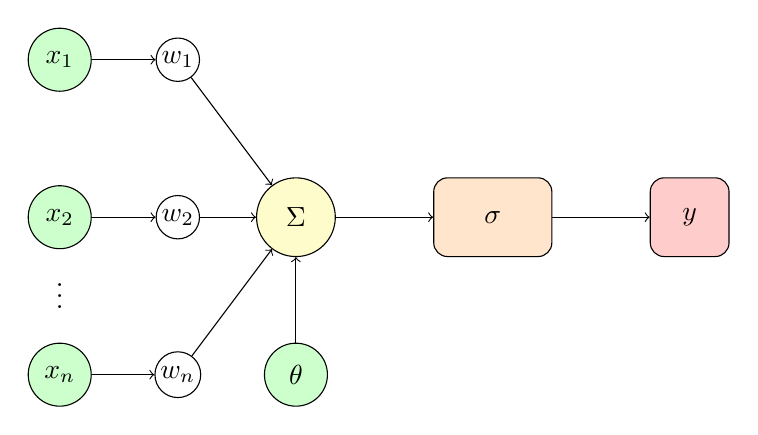
\begin{tikzpicture}[
    neuron/.style={circle, draw=black, fill=blue!20, minimum size=1.2cm},
    input/.style={circle, draw=black, fill=green!20, minimum size=0.8cm},
    weight/.style={fill=white, circle, draw=black, inner sep=1pt},
    arrow/.style={-Stealth, semithick},
    label/.style={text width=2cm, align=center, font=\small\sffamily}
]

\node[input] (x1) at (-3, 2) {$x_1$};
\node[input] (x2) at (-3, 0) {$x_2$};
\node at (-3, -0.9) {$\vdots$};
\node[input] (xn) at (-3, -2) {$x_n$};

\node[weight] (w1) at (-1.5, 2) {$w_1$};
\node[weight] (w2) at (-1.5, 0) {$w_2$};
\node[weight] (wn) at (-1.5, -2) {$w_n$};

\node[draw, circle, minimum size=1cm, fill=yellow!20] (sum) at (0, 0) {$\Sigma$};
\node[draw, rectangle, rounded corners=5pt, minimum width=1.5cm, minimum height=1cm, fill=orange!20] (act) at (2.5, 0) {$\sigma$};
\node[draw, rectangle, rounded corners=5pt, minimum width=1cm, minimum height=1cm, fill=red!20] (out) at (5, 0) {$y$};
\node[input] (b) at (0, -2) {$\theta$};

\draw (x1) edge[->] (w1);
\draw (x2) edge[->] (w2);
\draw (xn) edge[->] (wn);

\draw (w1) edge[->] (sum);
\draw (w2) edge[->] (sum);
\draw (wn) edge[->] (sum);

\draw (b) edge[->] (sum);
\draw (sum) edge[->] (act);
\draw (act) edge[->] (out);

\end{tikzpicture}
\caption{Representação gráfica de um neurónio de MacCough-Pitts. Fonte: elaborada pelos autores.}
\label{fig:neuronio-de-pitts}
\end{figure}

Formalizando matemáticamente a figura \ref{fig:neuronio-de-pitts},
sendo $W$ um vetor de pesos $\in [-1, 1]$, $\boldsymbol{x}$ um vetor de entradas
de tamanho $n$ e pertecente a $R^n$, $\theta$ um valor pertecente a $R$ 
e $\sigma$ uma função não linear. Um neurõnio é uma função $f: R^n \rightarrow R$,

\begin{eqnarray}\label{eq:neuronio-pitts}
    \sigma((\sum_{i=1}^{n} W_i\boldsymbol{x_i}) + \theta)
\end{eqnarray}

O termo $\theta$ pode ser entendido como o último elemento de $\boldsymbol{x}$ 
que está sendo sempre multiplicado pelo último elemento de $W$
que sempre tem valor igual a $1$, logo a equação \ref{eq:neuronio-pitts}
pode ser simplicada como,

\begin{eqnarray}\label{eq:neuronio-pitts-simplificado}
    \sigma(W\boldsymbol{x})
\end{eqnarray}

Um neurõnio pode ser entendido como uma transformação linear, a multiplicação
das entradas pelos pesos e viéses somados, seguida por uma
transformação não linear. Esta é feita pela função de ativação $\sigma$.
Alguns exemplos de funções de ativação empregradas nas redes neurais são A
função \textit{sigmoid} \ref{eq:sigmoid}, 
tangente hiperbólica (\textit{tanh}) \ref{eq:tanh}e 
\textit{Rectfied Linear Unit} (\textit{ReLU}) \ref{eq:relu}.

\begin{eqnarray}
    \text{sigmoid}(x) &=& \frac{e^x}{1 + e^x}\label{eq:sigmoid}
    \\
    \text{tanh}(x) &=& \frac{e^x - e^{-x}}{e^x + e^{-x}}\label{eq:tanh}
    \\ 
    \text{ReLU}(x) &=& \begin{cases} 
                        x & \text{if } x > 0 \\
                        0 & \text{if } x \leq 0 
                    \end{cases}\label{eq:relu}
\end{eqnarray}

Um único neurõnio não é capaz de aproximar qualquer função, para isso, eles são 
organizados em camadas que a saída de cada neurõnio de uma camada forma 
parte da entrada de todos os neurõnios da camada seguinte. 
A primeira camada apenas representa os dados de entrada, a última camada
representa um vetor de saída de tamanho 
Logo, uma rede neural \textit{feedfoward} com $L$ camadas escondidas 
pode ser entendida como uma função composta $f$ formada por 
um conjunto de consecutivas transformações lineares e não lineares num 
vetor de dados de entrada de tamanho $n$ $\boldsymbol{x} \in R^n$
que produz como saída um vetor de tamanho $m$ $\boldsymbol{\hat{y}} \in R^m$,  
sendo as transformações intermediárias representadas pelas saídas $y^l$ 
da camada escondida $l$, $l \in [1,..,L]$,

\begin{equation}\label{eq:rede-neural-composta}
    f(\boldsymbol{x}) = \sigma^{L + 1} y^{L + 1} \circ \sigma^{L} \circ y^{L} 
    \dots \circ \sigma^{2} \circ y^{2} \circ \sigma^{1} \circ y^{1}
\end{equation}

A figura \ref{fig:feedfoward-representacao-grafica} resume graficamente a
definição presente na equação \ref{eq:rede-neural-composta}.

\begin{figure}[htpb]
\centering
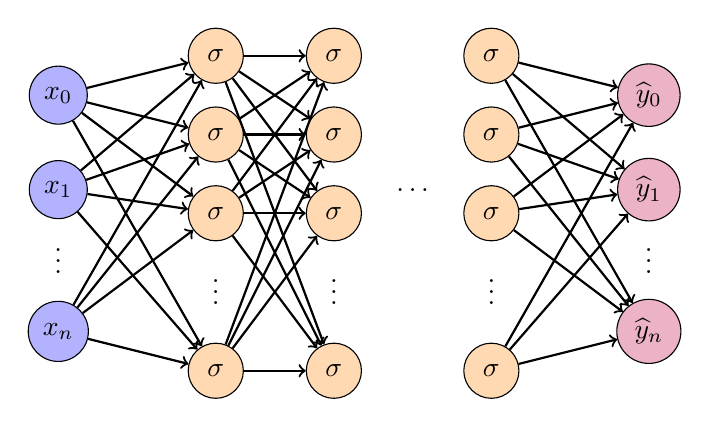
\begin{tikzpicture}[
    neuron/.style={circle, draw, minimum size=0.7cm},
    layer/.style={rectangle, minimum width=1.5cm, minimum height=8cm, draw=black, fill=blue!10, rounded corners=3pt},
    input/.style={neuron, fill=blue!30},
    hidden/.style={neuron, fill=orange!30},
    output/.style={neuron, fill=purple!30},
    physnode/.style={rectangle, draw, rounded corners, fill=orange!30, minimum width=1.5cm, minimum height=1.8cm},
    lossnode/.style={rectangle, draw, rounded corners, fill=yellow!30, minimum width=2cm, minimum height=3.2cm, align=center},
    every edge/.style={draw, ->, thick}
]

\node[input] (I-1) at (0, 3.5) {$x_0$};
\node[input] (I-2) at (0, 2.3) {$x_1$};
\node at (0, 1.5) {$\vdots$};
\node[input] (I-3) at (0, 0.5) {$x_n$};

\node[hidden] (H1-1) at (2, 4) {$\sigma$};
\node[hidden] (H1-2) at (2, 3) {$\sigma$};
\node[hidden] (H1-3) at (2, 2) {$\sigma$};
\node at (2, 1.1) {$\vdots$};
\node[hidden] (H1-4) at (2, 0) {$\sigma$};

\node[hidden] (H2-1) at (3.5, 4) {$\sigma$};
\node[hidden] (H2-2) at (3.5, 3) {$\sigma$};
\node[hidden] (H2-3) at (3.5, 2) {$\sigma$};
\node at (3.5, 1.1) {$\vdots$};
\node[hidden] (H2-4) at (3.5, 0) {$\sigma$};

\node at (4.5, 2.3) {$\dots$};

\node[hidden] (Hn-1) at (5.5, 4) {$\sigma$};
\node[hidden] (Hn-2) at (5.5, 3) {$\sigma$};
\node[hidden] (Hn-3) at (5.5, 2) {$\sigma$};
\node at (5.5, 1.1) {$\vdots$};
\node[hidden] (Hn-4) at (5.5, 0) {$\sigma$};

\node[output] (O-1) at (7.5, 3.5) {$\widehat{y}_0$};
\node[output] (O-2) at (7.5, 2.3) {$\widehat{y}_1$};
\node at (7.5, 1.5) {$\vdots$};
\node[output] (O-3) at (7.5, 0.5) {$\widehat{y}_n$};

% Connections
\foreach \i in {1,2,3}
    \foreach \j in {1,...,4}
        \path (I-\i) edge (H1-\j);

\foreach \i in {1,...,4}
    \foreach \j in {1,...,4}
        \path (H1-\i) edge (H2-\j);

\foreach \i in {1,...,4}
    \foreach \j in {1,...,3}
        \path (Hn-\i) edge (O-\j);

\end{tikzpicture}
\caption{Representação gráfica das redes \textit{feedfoward}. Fonte: elaborada pelos autores.}
\label{fig:feedfoward-representacao-grafica}
\end{figure}

O vetor de saída $\boldsymbol{\hat{y}}$ é então comparado com um vetor desejado 
$\boldsymbol{y}$ para calcular o erro entre a saída da rede e a saída desejada.
Este é o papel da função de perda (\textit{loss function}). 
Usualmente, para o caso de uma regressão, emprega-se a função de erro quadrático médio, 
do inglês, \textit{mean root square} (\textit{MSE}), como definida na equação
\ref{eq:mse}.

\begin{equation}\label{eq:mse}
    \mathcal{L} = MSE = \frac{1}{N} \sum_{i=0}^{N}(y_i - \hat{y}_i)^{2}
\end{equation}

Para problemas de classificação de classificação, aplica-se a função de entropia
cruzada \textit{cross-entropy} \ref{eq:cross-entropy} para problemas de 
classificação binária.

\begin{equation}\label{eq:cross-entropy}
    \mathcal{L} = MSE = - \sum_{i=0}^{N}(\frac{1}{N} y_i - \hat{y}_i)^{2}
\end{equation}

Já para o caso de classificação com multiplos rótulos, aplica-se e a função 
de \textit{softmax} \ref{eq:softmax}.

\begin{eqnarray}
    \rho_i &=& \frac{e^{z_i}}{\sum_{i=0}^{N}e^{z_j}} \\
    \mathcal{L} &=& arg max (\rho_0, \rho_1, \cdots, \rho_r) \label{eq:softmax}
\end{eqnarray}

A atualização dos pesos de cada camada se dá pela cálculo do grandiente
de uma função de erro $\mathcal{L}$. O "tamanho do passo" que será dado
é determinado por um parâmetro $\alpha$ chamado de taxa de aprendizagem.

\begin{eqnarray}\label{eq:atualizacao-parametros-redes}
    W_i^{t + 1} = W_i^{t} + \alpha \nabla \mathcal{L}
\end{eqnarray}

A propagação dos erros se dá pelo algoritmo de retropropagação, sendo um caso 
de aplicação da regra da cadeia. A derivada da 

\begin{equation}\label{eq:derivida-loss}
    \frac{d\mathcal{L}}{d\sigma^{L}} \cdot 
    \frac{d\sigma^{L}}{d\sigma^{L}} \cdot
    \cdots
\end{equation}



\section{Redes Neurais Informadas pela Física}

Apresentadas em \cite{raissi-etal:19}, PINNs podem ser entendidas como uma forma
avançada de regularização, ou como um problema de otimização que transforma 
as condições de fronteira e iniciais em penalizações para a função custo. 

\subsection{PINNs como Solucionadores de Equações Diferenciais}

PINNs são capazes de resolver problemas no seguinte formato: 

\begin{eqnarray}
    \mathcal{D}(u(\boldsymbol{x},t);\boldsymbol{\lambda}) &=& f(u,\boldsymbol{x},t), \quad \boldsymbol{x} \in \Omega, \, t \in I, \label{model-1-a}\\
    %
    \mathcal{B}(u(\boldsymbol{x},t)) &=& g(\boldsymbol{x},t), \quad \boldsymbol{x} \in \Gamma, \, t \in I, \label{model-1-b}\\
    %
    \mathcal{I}(u(\boldsymbol{x},t_0)) &=& q(\boldsymbol{x}), \quad \boldsymbol{x} \in \Omega, \label{model-1-c}
\end{eqnarray}

Em que $\Omega \subset \mathbb{R}^d$ é o domínio espacial limitado pela 
fronteira $\Gamma$; 
$d$ é a dimensão do domínio espacial; 
$T = [t_0, t_f]$ é o intervalo de tempo, sendo $t_0 < t_f$; 
$\boldsymbol{x} = (x_1, x_2, \dots, x_d)$ é um vetor de coordenadas espaciais; 
$t$ denota o tempo; 
$u = u(\boldsymbol{x}, t)$ denota a solução desconhecida do problema; 
$\boldsymbol{\lambda}$ é um vetor de parâmetros das equações; 
$\mathcal{D}$ é um operador diferencias associado às equações; 
$f$ é um termo fonte ou sorvedouro; 
$\mathcal{B}$ and $\mathcal{I}$ são operadores representando, respectivamente,
as condições de fronteira e iniciais; 
por fim, $g$ e $q$ são funções conhecidas que definem essas condições.

A equação \ref{eq:loss-fisica} define o termo da função de perda que engobla
todos as equações que compõem o modelo. Trata-se de um treinamento 
não-supervisionado que busca minimizar o residual definido.

\begin{equation}\label{eq:loss-fisica}
    \mathcal{L}_{\text{física}}(\boldsymbol{\theta}) 
    = \mathcal{L}_{\mathcal{D}}(\boldsymbol{x},t,\boldsymbol{\theta}) 
    + \mathcal{L}_{\mathcal{B}}(\boldsymbol{x},t,\boldsymbol{\theta}) 
    + \mathcal{L}_{\mathcal{I}}(\boldsymbol{x},t_0,\boldsymbol{\theta}) 
    %+ \omega_{data} J_{data}(\boldsymbol{x},t,\boldsymbol{\theta})
\end{equation}

Sendo $\omega_{\text{domínio}}$, $\omega_{\text{fronteira}}$ 
e $\omega_{\text{inicial}}$ pesos atribuídos a cada um dos residuais.
Caso haja dados disponíveis, é feito um treinamento supervisionado utilizando 
tais dados. A função de perda final da rede neural é então definida pela equação
\ref{eq:loss-total}.

\begin{eqnarray}\label{eq:loss-total} 
    \mathcal{L}_{\text{total}}(\boldsymbol{\theta}) 
    = \omega_{\text{física}} \mathcal{L}_{\text{física}}(\boldsymbol{\theta}) 
    + \omega_{\text{dados}} \,\mathcal{L}_{\text{dados}}(\boldsymbol{\theta})
\end{eqnarray}

Aqui vale menciona que esta não é a única forma de distribuir os pesos da loss,
a implementação da biblioteca \textit{DeepXDE} \cite{lu-etal:21-deepxde}
permite atribuir pesos diferentes a cada condição inicial e de fronteira. 
Então o problema passa a ser encontrar os conjuntos $\boldsymbol{\theta}^*$ de 
parâmetros e viéses da rede que minimiza a função \ref{eq:loss-total}.

\begin{equation}\label{eq:otimizacao-parametros}
   \boldsymbol{\theta}^* 
   = \arg \min_{\boldsymbol{\theta}} \mathcal{L}_{\text{total}}(\boldsymbol{\theta}), 
\end{equation}

Existem muitos métodos de otimização para encontrar os argumentos 
da equação \ref{eq:otimizacao-parametros}. Pode-se citar o método de 
primeira ordem \textit{Adam} \cite{kingma-ba:14-adam} e o método quase-newtoniano
\textit{BFGS}, ou como comumente usado, a sua versão para ambientes de pouca
memória, o \textit{L-BFGS} \cite{liu-nocedal:89-lbfgs}.

A figura \ref{fig:pinn-representacao-grafica} mostra uma representação gráfica das 
PINNs.

\begin{figure}[htpb]
\centering
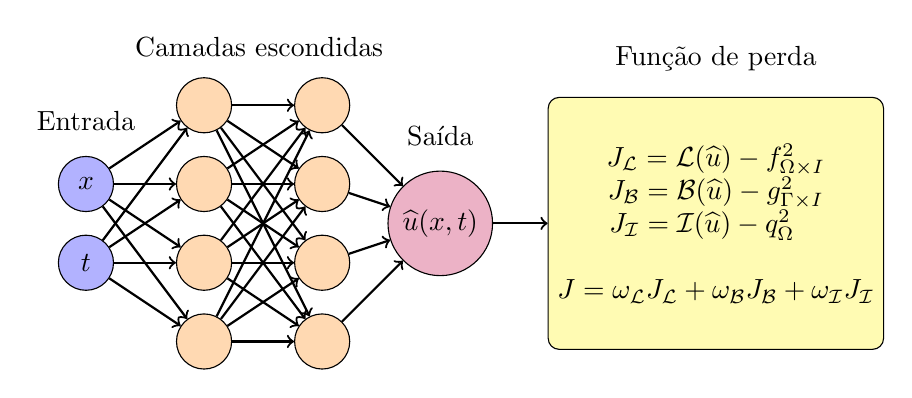
\begin{tikzpicture}[
    neuron/.style={circle, draw, minimum size=0.7cm},
    input/.style={neuron, fill=blue!30},
    hidden/.style={neuron, fill=orange!30},
    output/.style={neuron, fill=purple!30},
    physnode/.style={rectangle, draw, rounded corners, fill=orange!30, minimum width=1.5cm, minimum height=1.8cm},
    lossnode/.style={rectangle, draw, rounded corners, fill=yellow!30, minimum width=2cm, minimum height=3.2cm, align=center},
    every edge/.style={draw, ->, thick}
]

\node[input] (I-1) at (0, 2) {$x$};
\node[input] (I-2) at (0, 1) {$t$};

\node[hidden] (H1-1) at (1.5, 3) {};
\node[hidden] (H1-2) at (1.5, 2) {};
\node[hidden] (H1-3) at (1.5, 1) {};
\node[hidden] (H1-4) at (1.5, 0) {};

\node[hidden] (H2-1) at (3, 3) {};
\node[hidden] (H2-2) at (3, 2) {};
\node[hidden] (H2-3) at (3, 1) {};
\node[hidden] (H2-4) at (3, 0) {};

\node[output] (O-1) at (4.5, 1.5) {$\widehat{u}(x,t)$};

% Connections
\foreach \i in {1,2}
    \foreach \j in {1,...,4}
        \path (I-\i) edge (H1-\j);

\foreach \i in {1,...,4}
    \foreach \j in {1,...,4}
        \path (H1-\i) edge (H2-\j);

\foreach \j in {1,...,4}
    \path (H2-\j) edge (O-1);

\node[lossnode] (TotalLoss) at (8, 1.5) {
$J_{\mathcal{L}} = \lVert \mathcal{L}(\widehat{u}) - f \rVert^{2}_{\Omega \times I}$
\\
$J_{\mathcal{B}} = \lVert \mathcal{B}(\widehat{u}) - g \rVert^{2}_{\Gamma \times I}$
\\
$J_{\mathcal{I}} = \lVert \mathcal{I}(\widehat{u}) - q \rVert^{2}_{\Omega} \quad$
\\
\\
$J = \omega_{\mathcal{L}} J_{\mathcal{L}} + \omega_{\mathcal{B}} J_{\mathcal{B}} + \omega_{\mathcal{I}} J_{\mathcal{I}}$
};

\path (O-1) edge (TotalLoss);

% Labels
\node[above=0.2cm] at (I-1.north) {Entrada};
\node[above=0.2cm] at (2.2, 3.3) {Camadas escondidas};
\node[above=0.2cm] at (O-1.north) {Saída};
\node[above=0.2cm] at (TotalLoss.north) {Função de perda};

\end{tikzpicture}
\caption{Representação gráfica das PINNs. Fonte: elaborada pelos autores.}
\label{fig:pinn-representacao-grafica}
\end{figure}

\subsection{Formulação para Problemas Inversos}

A formulação para as PINNs apresentada até então foca na resolução de problemas
diretos. Em \cite{raissi-etal:19} é apresentada uma extensão para a mesma que 
também soluciona problemas inversos. Solucionar um problema inverso consiste em,
dado um conjunto de dados representados pela $\mathcal{L}_{\text{dados}}$,
encontrar um conjunto de parâmetros $\boldsymbol{\lambda}$ que minimaniza a
$\mathcal{L}_{\text{total}}$.
A equação \ref{eq:loss-total} pode então ser reescrita como,

\begin{eqnarray}\label{eq:loss-total-problema-inverso} 
    \mathcal{L}_{\text{total}}(\boldsymbol{\theta}, \boldsymbol{\lambda}) 
    = \omega_{\text{física}} \mathcal{L}_{\text{física}}(\boldsymbol{\theta}, \boldsymbol{\lambda}) 
    + \omega_{\text{dados}} \,\mathcal{L}_{\text{dados}}(\boldsymbol{\theta})
\end{eqnarray}

O problema de minimização descrito em \ref{eq:otimizacao-parametros} passa 
então a ser encontrar o conjunto $\boldsymbol{\theta}^*$ de parâmetros da rede,
como também o conjunto $\boldsymbol{\lambda}^*$
que minimiza a função \ref{eq:loss-total-problema-inverso}, 

\begin{equation}\label{eq:otimizacao-parametros-problema-inverso}
   (\boldsymbol{\theta}^*, \boldsymbol{\lambda}^*) 
   = \arg \min_{\boldsymbol{\theta}, \boldsymbol{\lambda}} \mathcal{L}_{\text{total}}(\boldsymbol{\theta}, \boldsymbol{\lambda}), 
\end{equation}

Vale salientar que a rede ao encontrar os conjuntos $\boldsymbol{\theta}^*$
e $\boldsymbol{\lambda}^*$, a rede neral está solucionando tanto o problema
direto (aproximar uma função que satisfaça as equações diferencias), quanto o 
problema inverso (encontrar $\boldsymbol{\lambda}^*$). 

\subsection{Pontos de Colocação}

Pontos de colocação são um conceito importante para as PINNs, sendo análogos
a criação da malha do \textit{MEF}. Entretanto, diferente do \textit{MEF}, 
não há um critério método bem definido para a obtenção destes pontos. 
Os pontos de colocação podem ser entendidos como uma discretização do domínio
de uma equação diferencial. O único critério que deve ser atendido é o uso
de pontos nas condições de fronteira e iniciais do problema.
Por esta perspectiva, os pontos de colocação podem ser entendidos como uma 
amostra do domínio na qual a rede neural será treinada. 
Por este motivo, muitas técnicas de amostragem multidimensional são 
aplicadas às PINNs para definir os pontos de colocação, pode-se citar como 
exemplo o hipercubo latino.

\section{Arquiteturas Alternativas}

A definição de PINNs como uma rede neural com informação física não se aplica
apenas a redes \textit{feedfoward}, qualquer arquitetura de redes neurais
que incorpora as equações que descrevem os dados em que rede está sendo treinada, 
pode ser considerada uma rede neural informada pela física, uma PINN.
Desde a publicação do artigo seminal em 2019, uma série de arquiteturas 
alternativas foram propostas utilizando a ideia das PINNs como princípio.

Uma classe de EDPs de especial interesse para áreas como teoria dos campos quânticos
e mecânica estatística são as EDPs estocásticas. Esta classe de equações diferenciais
pode ser entendida como uma equação diferencial com um termo $\xi$ que representa
um campo com ruído. 
O exemplo mais simples é a equação do calor estocástica \ref{eq:difusao-estocastica}.
\begin{equation}\label{eq:difusao-estocastica}
    \frac{\partial u}{\partial t} = \nabla \cdot u + \xi
\end{equation}
Uma proposta de PINNs para EDPs estocásticas é apresentada em \cite{zhang-etal:2020-stochastic-pde-pinns},
em que são empregados métodos espectrais ortogonais para modelar processos que 
representam a estocasticidade nos dados. Estes processos são incorporados à função 
de perda como termos regularizadores extras.  
Outra arquitetura pensada para a solução de EDPs estocásticas são as FINNs,
apresentadas em \cite{karlbauer-2022-finns}, que combinam o método de volumes finitos
com redes neurais para obter soluções para problemas de advecção-difusão como a
equação de \textit{Burgers} e de \textit{Allen-Cahn}.
A arquitetura obteve resultados superiores a redes neurais sem informação física
e até mesmo de PINNs convencionais.   

Um exemplo de proposta de PINNs alternativas que explora limitações das PINNs 
originais pode ser encontrada em \cite{sun-e-feng:2023-gPINNs}.
Os autores propõem as gPINNs (Gradient Enhanced PINNs) que tentam contornar as 
complexidades dos algoritmos de diferenciação automática existentes para equações de alta 
ordem. A arquitetura utiliza uma função de ativação adaptativa, uma técnica de 
melhoria nos gradientes para acelerar a convergência do modelo, e uma técnica 
chamada de \textit{deep mixed residual method} para compensar o \textit{overhead}
gerado pela melhoria nos gradientes. A arquitetura é empregada na solução de 
equações de onda da luz.
Outra proposta similar que também explora o uso de melhorias no gradientes pode 
ser encontrada em \cite{mohammadian-etal:2023-gradient-enhanced}, tendo como
maior vantagem a necessidade de poucos dados para treinamento, acelerando o processo
de treinamento.
Os autores utilizam o método proposto para gerar estimativas para sistemas de 
controle de redes elétricas.  

Técnicas como convolução e recorrência, comuns em áreas como visão computacional 
e processamento de linguagem natural, também encontram espaço na solução de problemas
científicos. Em \cite{ren-etal:2022-phycrnet} são propostas as PhyCRNet e PhyCRNet-s
para resolução de EDPs sem dados de treinamento. A arquitetura emprega uma rede
LSTM \textit{enconder-decoder} com convolução para a extração de características
espaciais e simulação da evolução do fenômeno no tempo.
Para evitar o ajuste de hiper-parâmetros, as condições iniciais e de contorno não
são impostas por meio de penaliadades na função custo, mas como \textit{hard-constraints}.
Também são utilizadas conexões residuais e autoregressivas para simular a progressão
do tempo. OS autores obtiveram resultados satisfatórios para problemas como a 
equação de \textit{Burgers} e problemas de reação-difusão.
Outro exemplo envolvendo camadas convolucionais pode ser encontrado em 
\cite{shi-etal:24-convnet}. No artigo é proposto uma arquitetura em que uma única 
camada convolucional é empregada. Nos testes realizados pelos autores, a rede 
neural proposta apresentou uma convergência melhor do que uma PINN convecional 
para problemas de difusão com diferentes frequências.

Pensanda para lidar com problemas ligadas a solução de PDEs com dados que possuem 
componentes com fequências diferentes, a arquitetura proposta em \cite{han-etal:2023-hierarchical-learning}
utiliza aprendizado hierarquico para lidar com esse problema.
O princípio por de trás do aprendizado hierarquico é utilizar camadas com redes
neurais responsáveis por aproximar uma frequência, assim cada camada 
adicionada deve aprender a partir dos dados residuais da camada anterior.
A saída dessas camadas é então alimentada em uma rede de características de Fourier
embutidas. 
As primeiras camadas capturam os componentes de menor frequência, enquanto que
que a rede de características embutidas fica responsável por impor limites a solução.
A arquitetura proposta é testada com uma série de equações diferenciais parciais.

Outro exemplo de arquiteturas alternativas de redes neurais com informação física
pode ser encontrada em \cite{benjamin-etal:2022-rnn-dct-networks}. 
Os autores propoêm as \textit{rnn-dct networks}, que combinam a arquitetura clássica
de redes residuais (RNN) e DCT (\textit{discrete cossine transformations}) com 
redes MLP (feedfoward). O DCT é responsável por codificar a parte espacial da equação,
enquanto que a RNN fica responsável por interpretar os valores temporais.
O resultado dessas duas redes são então combinados e usados para alimentar a rede
\textit{feedfoward}, ajudando esta a capturar as relações espaciais e temporais do
problema. A arquitetura proposta apresentou resultados execelentes em problemas 
envolvendo as equações de Navier-Stokes, como o problema de vortices de Taylor-Green.

Em \cite{pakravan-et:2021-bipde} é apresentado um método focado na solução de 
problemos inversos envolvendo EDPs com lacunas nos dados chamado 
\textit{Blended inverse-PDE networks} BiPDE.
Os parâmetros da equação são descobertos utilizando não apenas conhecimentos sobre
a física incorporados a função de perda, mas também utilizando conhecimentos específicos 
do domínio. 
A rede neural exerce o papel de aproximador universal dos parâmetros, que combinado 
com um solucionador de EDPs, livra a rede de ter que resolver o problema de 
forma direta, focando apenas no problema inverso, tornando o método mais eficiente,
ao não necessitar de tantos dados para o treinamento.
O método proposto é testado em problemas inversos envolvendo encontrar coeficientes
de difusão variantes para as equações de \textit{Burgers} e de \textit{Poisson}, 
além de problemas de alta dimensionalidade.

Propostas em \cite{jagtap-etal:2020-convervative-pinns}, as conservative PINNs 
(cPINNs) utilizam leis de conservação não-lineares para a solução de problemas 
em domínios discretos. Para aplicar as cPINNs, o domínio é fragmentado em subdomínios
nos quais as cPINNs aão empregadas, a propriedade de conversão é garantida pela 
aplicação de continuidade ao longo de todos os subdomínios. Nas fronteiras entre
os subdomínios, a solução é obtida pela média das saídas de cada cPINN.
Uma vantagem desta arquitetura é permitir que em cada subdomínio sejam utilizados
diferentes meta-parãmetros, como número de camadas escondidas, funcões de ativação
e otimizadores.
A arquitetura é capaz de tirar grade proveito de processamento paralelo.  

Utilizando as cPINNs como base, as \textit{Extended Physics-informed Neural Networks}
(XPINNs) são propostas em \cite{jagtap-etal:2020-extended-pinns}. Assim como as 
cPINNs, o domínio é fragmentado em subdomínios permetindo que a otimização dos
meta-parâmetros possa ser feita em cada rede. 
A grande novidade da arquitetura é a possibilidade de aproximar qualquer EDP.
Outra novidade é a decomposição arbritária do domínio, o que permite tirar ainda
mais profeito de paralelismo durante o treinamento do modelo.
A arquitetura foi aplicada em PDE não-lineares com geometrias complexas, 
aproveitando a decomposição de domínio.
Continuando o desenvolvimento da arquitetura, em \cite{hu-etal:2023-augmented-pinns}
são propostas as \textit{Augmented PINNs} (APINNs), a novidade da arquitetura 
é tornar a fragmentação dos subdomínios treinável.
A arquitetura permite que dados de treinamento sejam usados entre diferentes 
fragmentos, aumentando a generalização do modelo.
A performance das APINNs é consideravelmente superior a das XPINNs em termos 
de fragmentação do domínio e generalização.

Aproveitando as possibilidades que o uso de paralelismo pode trazer em termos 
de velocindade no tempo de treinamento, em \cite{dwivedi:2019-distributed-pinns}
são propostas as Distribuited PINNs (DPINNs). A principal ideia por trás deste método
é fragmentar o domínio do problema em partes que devem ser aproximadas por uma rede
neural independente. Uma vantagem dessa abordagem é que é possível utilizar redes
mais simples em cada fragmento, ao invés de aplicar uma única rede mais complexa
para todo o domínio. A função de perda é calculada com base na aproximação de cada
rede neural que funcionam como PINNs paralelas. O método é capaz de aproximar 
corretamente problemas difícies como as equações de Navier-Stokes de forma satisfatória
utilizando redes simples, obtendo resultados melhores do que aqueles com uma
rede neural informada pela física centralizada.

Problemas de engenharia costumam ter parâmetros incertos que são dependentes 
de variáveis temporais e espaciais, estas incertezas são contornadas utilizando
processos que as modelam.
Métodos como o MEF são capazes de resolver tais equações, mas é necessário ter um
conhecimento \textit{a priori} sobre as distribuições que modelam o fenômeno estudado,
fazendo com que métodos puramente estátiscos sejam insuficientes.
É comum empregar técnicas como teoria de conjuntos difusos junto aos métodos 
tradicionais de solução de equações diferenciais.
Aproveitando o potencial que as PINNs e conjuntos difusos tem para a soluções 
de equações com tais características, em \cite{fugh-etal:2022-fuzzy-pinns} 
são propostos dois novos modelos as 
\textit{Interval Physics-Informed Neural Networks} (iPINNs) e 
\textit{Fuzzy Physics-Informed Neural Networks} (fPINNs) que combinadas, 
são capazes de resolver problemas envolvendo equações diferencias e conjuntos 
difusos sem conhecimentos prévios. Uma rede neural é responsável pela a aproximação 
das entradas, enquanto a outra fica responsável por aproximar a solução da PDE.  
O método proposto mantêm as vantagens das PINNs, como não precisar de uma 
malha de pontos, e ser capaz de resolver problemas de forma direta e inversa
sem alterações significativas nos métodos.

As equações de ordem fracionaria, também chamadas de equações diferenciais 
extraordinárias, são uma classe de equações diferencias que encontram aplicações 
na modelagem de diversos fenõmenos físicos como escoamentos subterrâneos 
\cite{atangana-2013-fluxo-ordem-fracionaria} e equações de conservação de massa
\cite{wheatcraft-2008-conservacao-de-massa-fracionaria}. 
A equação \ref{eq:exemplo-ordem-fracionaria} mostra a forma geral para tais equações.
\begin{equation}\label{eq:exemplo-ordem-fracionaria}
    \dfrac{d^{\alpha}u}{dx^{\alpha}} = u, \quad \alpha \in \mathbb{R}
\end{equation}
Em \cite{pang-etal:2019-fPINNs} é proposto uma arquitetura de redes neurais 
informadas pela física pensada para equações diferenciais de ordem fracionária.
O principal entrave para o uso de PINNs convecionais na solução dessas equações
está ligado ao fato de que algoritmos de diferenciação automática são otimizados
para equações de ordem inteira.
A arquitetura proposta, chamado de \textit{fPINNs}, contorna tais limitações ao
aplicar uma abordagem mista que utiliza diferenciação automática para a parte inteira
das derivadas e derivadas númericas para a parte fracionária.
A arquitetura proposta foi capaz de solucionar problemas clássicos como a equação de 
\textit{Burgers} utilizando derivadas parciais de ordem fracionária, obtendo
resultados equiparáveis ao MEF.

% Em \cite{sirignano-spiliopoulos:2018-deepgalerkin} é proposto o 
% \textit{DeepGalerkin}, um método sem malhas para a solução de equações
% diferencias de alta dimensionalidade que combina o método de Galerkin com
% redes neurais. 

Baseado nas \textit{KANs} (\textit{Kolmogorov-Arnold Neural Networks})
\cite{liu-etal:2025-kans}, redes neurais baseadas no teorema de representação 
universal de Kolmogorov-Arnold, foram propostas as \textit{PIKANs} 
(\textit{Physically Informed Kolmogorov-Arnold Neural Networks})
que combinando as funcões de ativação baseadas em \textit{b-splines} das
\textit{KANs} com a técnica de regressão simbólica, permite encontrar  
representações analíticas das soluções encontradas pela rede neural.
As KANs não se mostraram superiores aos MLPs para todo tipo de tarefa 
\cite{toscano:2025-pinns-para-pikans}, mas sua superiodade com regressão simbólica
demonstra o potencial da arquitetura para problemas envolvendo explicabilidade.

% \cite{toscano:2025-pinns-para-pikans}
